\documentclass{article}
\usepackage{graphicx} % Required for inserting images
\usepackage{amssymb}
\usepackage{amsmath}
\usepackage{bbm}
\usepackage{xcolor}

\title{CSE 222A Project Report}
\author{Ziyuan Lin}
\date{2024.12.2}

\begin{document}
\maketitle

\section{Github Link}
https://github.com/duckddclown/CSE-222A-Final.git

\section{Introduction}
$21^{st}$ centry has seen the fast development of the internet. Many congestion control algorithms are invented to balance the network traffic and improve the performance of the network.
Among congestion control algorithms, there are two main types. The first one is loss-based algorithms. These algorithms modify the window size based the signal of losses. The second kind is 
rate-based algorithms. These algorithms use the congestion signal inside the network, including latency, queuing delay at router, etc.
\\[6pt]
In the past ten years, cloud computing has become a very important method of computation. More and more companies are deploying their applications on cloud. Investigating congestion control
inside cloud becomes a desirable experiment. In particular, we want to investigate how Cubic(loss-based)[1] and BBR(rate-based)[2] algorithm performs on different applications in cloud. 

\section{Related Work}
In this section, we provide a review of how Cubic and BBR works. Cubic is a loss-based congestion control algorithm. It is a modified version of the reno TCP. Cubic mainly changes the AIMD phase
of reno. After multiplicative decrease, the cubic increase the congestion window increases as a "cubic" function with repect to time. It increases quite fast after immediate decrease and get slower.
Once the window size goes larger than the window size before the previous decrease, the window size growth gets larger again. BBR is a rate-based algorithm. BBR measures the minimum rtt and maximum
recent bandwidth to decide how should the congestion window change. BRR typically adjust more sensitive compared to loss-based algorithm.

\section{Process Overview and Experimental Methodology}
We choose amazon ec2 ubuntu as our experiment environment. We choose two applications to investigate the network behavior. The first one is iperf3, which is network testing tool involving bulk traffic.
It mimics the behavior of all large file transfer applications. In particular, the network behavior is "best effort" in the sense that the application does not limit the congestion window size. The other
application we choose is FFmpeg, a video streaming application. Video streaming is special because the its target is to present the fixed amount of data in a unit of time. The reciever may have a specialized queue to buffer
the coming streaming data. If this is the case, the application may restrict the congestion window size to avoid congestion in the buffer.
\\[6pt]
We create two ubuntu at different places serve as two nodes. One is sender $A$, and the other receiver $B$. We set up both iperf3 and FFmpeg as sender at $A$ and receiver at $B$. The location of two nodes are both at California.
We add a 20ms delay at the sender $A$ to create a bottleneck. Then we apply Cubic or BBR to the congestion control algorithm and measure different metrics of the application and network, including congestion window size(cwnd),
slow start threshold(ssthresh), throughput, etc. We use ss(socket statistics) tool to measure the network behavior in the background. We conduct iperf3 for 3000 ms. The video size is around 17500 ms. Then we manually introduce packets loss at sender $A$ and use ss to see how network behave under
the circumstance of packet loss.
\\[6pt]
All the work is done on my own account. I use the free tier one, so it only costs me $0.2$\$.

\section{Results and Explanation}
In this section, we provide the experiment result and explain why it behaves this way. 
\subsection{CWND and ssthresh Behavior of iperf3}
Figure $1$ shows how cwnd behave for iperf3.
\begin{figure}[h]
    \begin{minipage}[b]{0.45\textwidth}
        \centering
        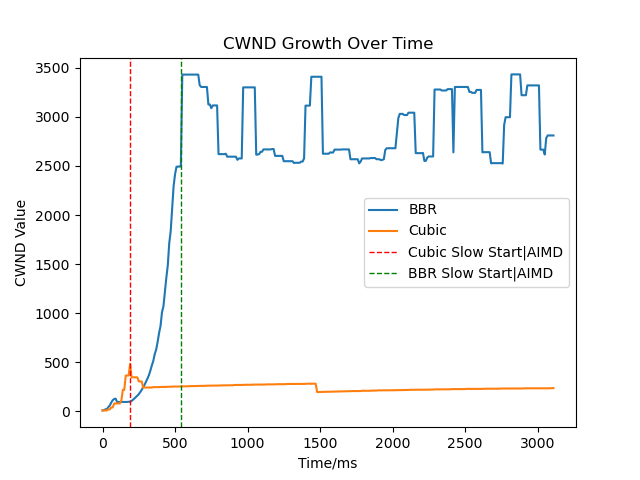
\includegraphics[width=\textwidth]{../figure/cwnd.png}
        \caption{How cwnd changes with repect to time}
        \label{fig:fig1}
    \end{minipage}
    \hfill
    \begin{minipage}[b]{0.45\textwidth}
        \centering
        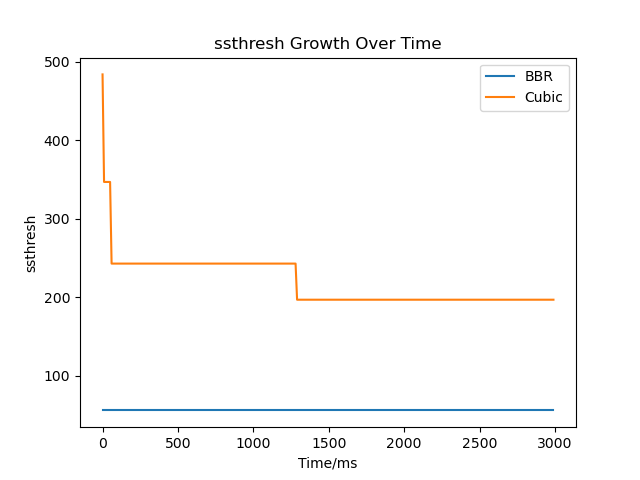
\includegraphics[width=\textwidth]{../figure/ssthresh.png}
        \caption{How ssthresh changes with repect to time}
        \label{fig:fig2}
    \end{minipage}
\end{figure}
\\[6pt]
The red(green) dashed vertical line separates the Cubic(BBR) slow start region(left) and smooth region(right). As we can see, Cubic's cwnd is much smaller compared to BBR.
The reason behind it relies on the natural difference between loss-based and rate-based protocol. Accidental packet loss or delay may cause a multiplicative decrease of cwnd.
Cubic cwnd recovers faster than reno, but can still be very slow at cwnd before decrease. However, BBR does not have such issue. rtt and bandwidth measurement instantly and smoothly reflect the current network behavior,
causing cwnd to quick adjust to the size that results in best performance without introducing the congestion. Also, notice that a sudden drop of bandwidth available or packet drop could cause a large decrease for Cubic and 
recovers slowly, while BBR can recover as soon as receiving the next rtt stats.
\\[6pt]
The ssthresh is shown in figure $2$. As we can see that ssthesh of BBR almost does not change. This is because ssthresh does not mean much for a rate-based protocol. Cubic's ssthresh changes due to accidental packet loss and delay.

\subsection{Network Analysis for iperf3}
We do the experiment for 5 times and the following are the average statistics. The throughput of Cubic is $78.6$ Mbits/sec. The throughput of BBR is $503 Mbits/sec$. As we can see the throughput of $BBR$ is almost $7$ times greater than
Cubic. The RTT of Cubic is $23.336$ ms. The RTT of BRR is $21.030$ ms. BBR is RTT-triggered, thus can keep the RTT very stable. Cubic is loss-triggered, the RTT may increase due to late discovery of loss.

\subsection{CWND and ssthresh Behavior under Packet Loss for iperf3}
Figure $3$ shows how cwnd behaves with different loss rate for Cubic. 
\begin{figure}[h]
    \begin{minipage}[b]{0.45\textwidth}
        \centering
        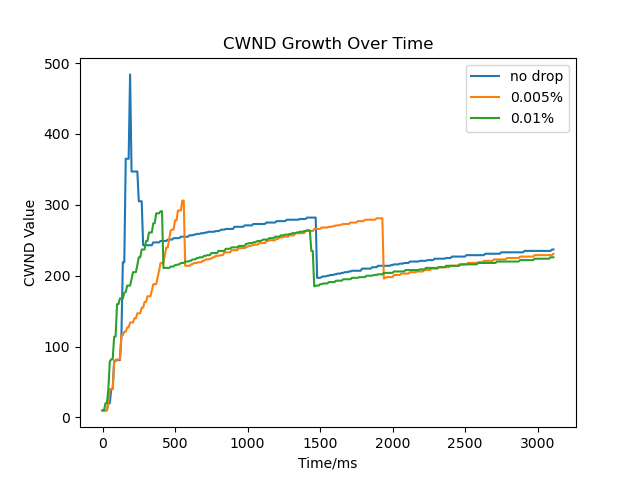
\includegraphics[width=\textwidth]{../figure/cubic_cwnd_drop.png}
        \caption{How cwnd changes with repect to time for Cubic}
        \label{fig:fig3}
    \end{minipage}
    \hfill
    \begin{minipage}[b]{0.45\textwidth}
        \centering
        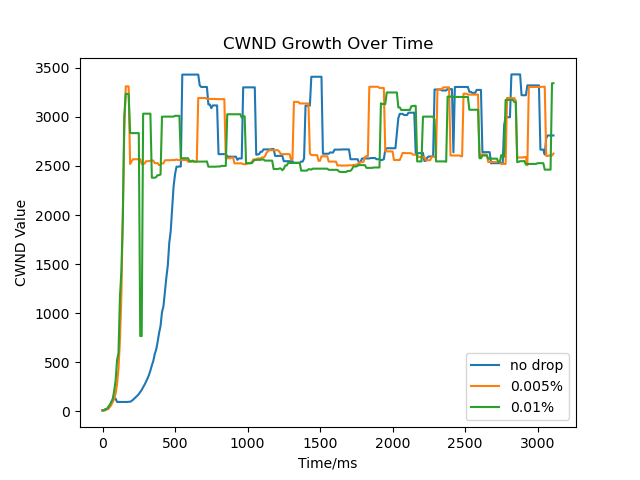
\includegraphics[width=\textwidth]{../figure/BBR_cwnd_drop.png}
        \caption{How cwnd changes with repect to time for BBR}
        \label{fig:fig4}
    \end{minipage}
\end{figure}
\\[6pt]
As we can see, manually increase loss rate could decrease cwnd for Cubic, which is due to its naturality of being loss-based protocol. The throughput of $0.005\%$ drop rate is $73.4$ Mbits/sec. The throughput of $0.01\%$ drop rate is $71.3$ Mbits/sec. I have also
implemented a loss rate of $0.1\%$, this cause the throughput to drop to $20.5$ Mbits/sec.
\\[6pt]
Figure $4$ shows how BBR is affected by packet loss. The throughput of $0.005\%$ drop rate is $570$ Mbits/sec. The throughput of $0.01\%$ drop rate is $553$ Mbits/sec. The throughput of $0.1\%$ drop rate is $540$ Mbits/sec. Consequently, we conclude that BBR is not
sensitive to packet loss due to the fact that packet loss cannot directly change the cwnd. The small decrease in throughput may due to retransmission.

\subsection{Fairness in iperf3}
We set two iperf3s $S_1,S_2$ on node $A$, and let them simultaneously tranmit packets to $B$. The results are as follows: the throughput for Cubic is $38.8$ Mbits/sec for $S_1$, 50.9 Mbits/sec for $S_2$. The throughput for BBR is 277 Mbits/sec for $S_1$ and 273 Mbits/sec
for $S_2$. Thus we conclude that BBR is more fair compared with Cubic. The reason for this is that BBR can detect the available bandwidth and adjust cwnd very fast, causing fast convergence. Cubic is loss-based, a packet loss may cause $S_2$ to loss lots of throughput, while
$S_1$ keep increasing.

\subsection{CWND and ssthresh Behavior of FFmpeg}
Figure 5 shows how cwnd changes in FFmpeg.
\begin{figure}[h]
    \centering
    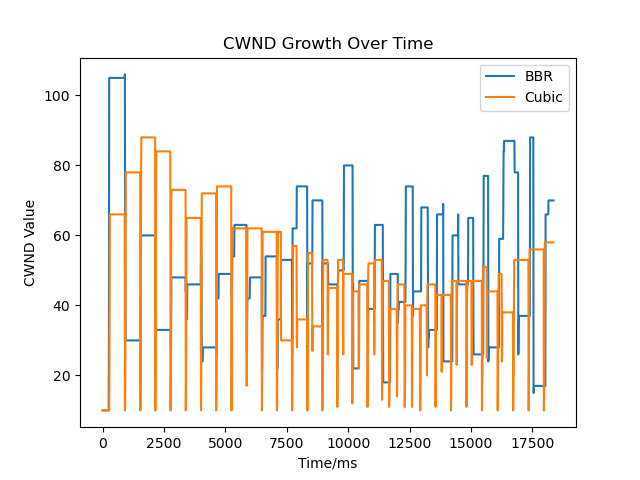
\includegraphics[width=0.7\textwidth]{../figure/video_cwnd.png}
    \caption{How cwnd changes with repect to time}
    \label{fig:fig5}
\end{figure}
\\[6pt]
In the video streaming context, the cwnd size is restricted. Since the main job of video streaming is not sending all data at the same time, FFmpeg does not perform "best effort" work. We guess this could due to two reasons. The first is that the small window size can optimize the entire network environment.
Since FFmpeg only need to ensure node $B$ can obtain the data it need for the future $2-3$ seconds, it can send slowly and give more bandwidth to other more urgent applications. This can also avoid burst of traffic. The other possible conjecture is that FFmpeg has a special queue for video streaming. In order
not to make queue full, it shrinks the cwnd to the minimum required. The ssthresh thus do not have much meaning in this context, so we do not provide it.
\subsection{Network Analysis for FFmpeg}
The throughput depends on the video we want to stream. For a 128 * 64, 30 fps video, the throughput is 735.0kbits/s for either protocol. The flow completion time of the video is 17820 ms. The RTT is 22.13 ms.
\subsection{CWND and Behavior under Packet Loss for FFmpeg}
Figure 6 shows how cwnd changes with respect to packet loss for Cubic. Figure 7 shows the cwnd changes with respect to packet loss for BRR.
\begin{figure}[h]
    \begin{minipage}[b]{0.45\textwidth}
        \centering
        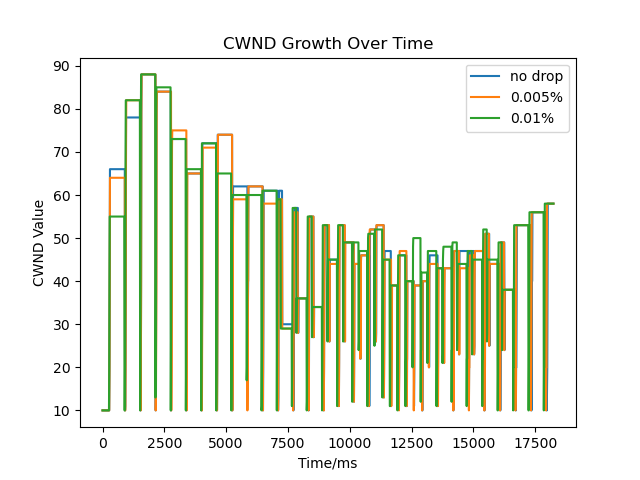
\includegraphics[width=\textwidth]{../figure/video_cubic_cwnd_drop.png}
        \caption{How cwnd changes with repect to time for Cubic}
        \label{fig:fig6}
    \end{minipage}
    \hfill
    \begin{minipage}[b]{0.45\textwidth}
        \centering
        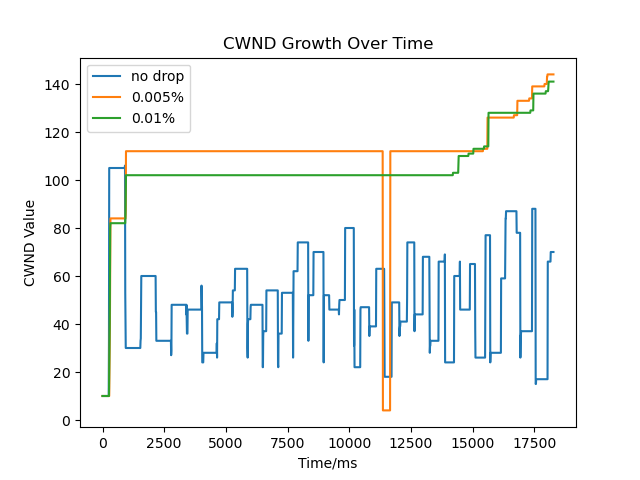
\includegraphics[width=\textwidth]{../figure/video_BBR_cwnd_drop.png}
        \caption{How cwnd changes with repect to time for BBR}
        \label{fig:fig7}
    \end{minipage}
\end{figure}
\\[6pt]
As we can see, Cubic and BBR video streaming are not sensitive to packet loss. The throughput does not change much. The application controls the cwnd size so that cwnd of Cubic does not decrease with packet drop.
\section{Conclusion}
In this project, we investigated how loss-based and rate-based network behave in the cloud compuitng environment. For iperf3 application, BBR performs much better than Cubic because the cwnd does not depend on packet loss.
For video streaming application, specific protocol will not change the throughput and cwnd significantly, mainly due to relative constant demand. We also investigate how different protocols acts under packet loss. For iperf3 application,
Cubic is much more sensitive to packet drop compared to BBR. Finally, we look at the fairness of different protocols. BBR provides much better fairness compared with Cubic.

\section{Reference}
[1]Ha, Sangtae, Injong Rhee, and Lisong Xu. "CUBIC: a new TCP-friendly high-speed TCP variant." ACM SIGOPS operating systems review 42.5 (2008): 64-74.
\\[6pt]
[2]Cardwell, Neal, et al. "Bbr: Congestion-based congestion control: Measuring bottleneck bandwidth and round-trip propagation time." Queue 14.5 (2016): 20-53.
\\[6pt]
\end{document}